\documentclass[11pt]{article}

\usepackage{amsmath,amssymb,amsthm}
\usepackage{enumitem}
\usepackage{tikz}
\usetikzlibrary{arrows.meta}

\setlength{\parindent}{0pt}
\setlist[enumerate,1]{label=\textbf{(\arabic*)}}
\setlist[enumerate,2]{label=\textbf{(\alph*)}}

\begin{document}

\begin{center}
{\Large \textbf{6.\ Problems}}
\end{center}

\begin{enumerate}

\item We will prove that all horses are the same color. To do this,
we will show that if we have any collection of $n \ge 1$ horses,
then all $n$ of these horses are the same color.

We begin with the base case, $n=1$. If we have only one
horse, then all the horses clearly have the same color.

Next, we do the inductive step. Suppose that $n$ horses are
always the same color. We will show that $n+1$ horses are always
the same color. Let us number the horses $H_1,\ldots,H_{n+1}$.
Since we are assuming that \emph{any} set of $n$ horses are the
same color, then $H_1,\ldots,H_n$ are the same color. Similarly,
$H_2,\ldots,H_{n+1}$ are the same color. Now, any horse in the middle
is the same color as both $H_1$ and $H_{n+1}$, so $H_1$ and $H_{n+1}$
are the same color. Thus all $n+1$ horses are the same color.\newline
What is the mistake in this argument?

\item What is the sum of the first $n$ odd numbers? Give a proof using induction.

\item Prove that
\[
1^3 + 2^3 + \cdots + n^3 \;=\; \frac{n^2(n+1)^2}{4} \;=\; (1+2+\cdots+n)^2.
\]
Then express this statement using $\Sigma$ notation, without the $\cdots$.

\item Prove that for every nonnegative integer $n$, the number $n^5-n$
is a multiple of $5$. What about for negative integers?

\item Prove that if $x>-1$ and $n$ is a nonnegative integer, then
$(1+x)^n \ge 1+nx$.

\item Let $F_n$ be the $n^{\text{th}}$ Fibonacci number, defined by $F_0=0$,
$F_1=1$, and $F_{n+2}=F_n+F_{n+1}$ for $n\ge 0$. Prove that
\[
F_n=\frac{1}{\sqrt{5}}\left(\left(\frac{1+\sqrt{5}}{2}\right)^{\!n}
-\left(\frac{1-\sqrt{5}}{2}\right)^{\!n}\right).
\]

\item Show that every positive integer $n$ can be written in the form
\[
n=a_1\cdot 1! + a_2\cdot 2! + a_3\cdot 3! + \cdots + a_k\cdot k!,
\]
where $k$ is a positive integer, each $a_i$ is a nonnegative integer,
and for all $i$ with $1\le i\le k$, we have $0\le a_i\le i$.

\item Prove that for all nonnegative integers $n$, a number consisting
of $3^n$ equal digits is divisible by $3^n$.

\item Prove that for every positive integer $n$, there exists an $n$-digit
number divisible by $5^n$ whose digits are all odd.

\item Prove that every positive integer $n\ge 1$ can be expressed as
a sum of pairwise nonconsecutive Fibonacci numbers. That
is, for every positive integer $n$, there is some positive integer
$k\ge 2$ and numbers $a_2,\ldots,a_k$ which are each either $0$ or $1$
such that
\[
n=\sum_{i=2}^k a_i F_i,
\]
and if $a_i=1$, then $a_{i-1}$ and $a_{i+1}$ must both be $0$.

\item The Ackermann function $A(m,n)$ is a function of two nonnegative
integer variables, defined by
\[
A(m,n)=
\begin{cases}
n+1, & m=0,\\[2pt]
A(m-1,1), & m>0\text{ and }n=0,\\[2pt]
A\bigl(m-1,\,A(m,n-1)\bigr), & m>0\text{ and }n>0.
\end{cases}
\]
For $m=0,1,2,3,4$, find and prove a formula for $A(m,n)$.
What about when $m=5$?

\item A \emph{graph} consists of a collection of vertices, drawn as dots,
together with edges, which connect pairs of edges. For a graph $G$,
let $C_G(n)$ denote the number of ways of coloring each vertex of $G$
using one of $n$ colors, such that if $v$ and $w$ are vertices connected
by an edge, then they are colored differently. The goal of this problem
is to prove some facts about the function $C_G(n)$.
\newline 
\begin{figure}[h]
\centering
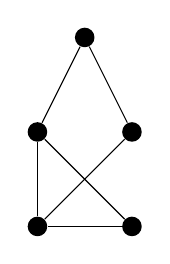
\begin{tikzpicture}[scale=1.2, every node/.style={circle, fill=black, inner sep=2.5pt}]
  % vertices
  \node (A) at (0,0)   {}; % bottom-left
  \node (B) at (1,0)   {}; % bottom-right
  \node (C) at (0,1) {}; % middle-left
  \node (D) at (1,1) {}; % middle-right
  \node (E) at (0.5,2) {}; % top

  % edges (exactly as in the figure)
  \draw (A)--(B);  % bottom edge
  \draw (A)--(C);  % left vertical
  \draw (C)--(E);  % left up-slant
  \draw (D)--(E);  % right up-slant
  \draw (C)--(B);  % down-right diagonal
  \draw (D)--(A);  % down-left diagonal
\end{tikzpicture}

\medskip
\caption{A graph.}
\end{figure}


\begin{enumerate}
\item Let $e$ be an edge of a graph $G$. We define the \emph{deletion} of
$e$ to be the graph $G\setminus e$, which is the same as $G$ except with edge $e$
deleted. We also define the \emph{contraction} of $e$ to be the graph $G/e$,
which is the same as $G$ except that the edge $e$ is deleted and the two endpoints of $e$
are glued together. Prove that $C_G(n)=C_{G\setminus e}(n)-C_{G/e}(n)$.
This is known as the \emph{deletion--contraction formula}. This
formula will be helpful for the later parts of this problem.

\item Prove that, for any graph $G$, $C_G(n)$ is a polynomial function of $n$.
(Hint: Use induction on the number of vertices plus the number of edges of $G$.)

\item Prove that the degree of the polynomial $C_G(n)$ is equal to the number of vertices of $G$.

\item Suppose that $C_G(n)=\sum_{i=0}^k a_i n^i$. Prove that the signs
of the coefficients $a_i$ alternate: if $k$ is the degree of $C_G(n)$,
then $a_k>0$, $a_{k-1}\le 0$, $a_{k-2}\ge 0$, $a_{k-3}\le 0$, and so forth.
\end{enumerate}

\end{enumerate}

\end{document}
